% V-образные слои модифицированного алгоритма (рис. к подразделу
% «Модифицированный алгоритм»). Единица координат = ширина белого ромба.
% Заземлённый ромб G(x,s): нижний (x,0.5), левый (x-s/2,0.5+s/2),
% правый (x+s/2,0.5+s/2), верхний (x,0.5+s). Шеврон C(x,s) = G(x,2s)\G(x,s)
% -- шестиугольник L_i -> L_o -> T_o -> R_o -> R_i -> T_i, где
% L_i=(x-s/2,0.5+s/2), L_o=(x-s,0.5+s), T_o=(x,0.5+2s),
% R_o=(x+s,0.5+s), R_i=(x+s/2,0.5+s/2), T_i=(x,0.5+s).
% Все фигуры обрезаны по треугольнику таблицы.
% Цвета слоёв -- полупрозрачные заливки оригинального изображения
% (alpha = 99/255), скомпозитированные на белый фон.
\definecolor{LayerPink}{HTML}{ffaeee}
\definecolor{LayerGray}{HTML}{c7d2d4}
\definecolor{LayerOrange}{HTML}{eebd9c}

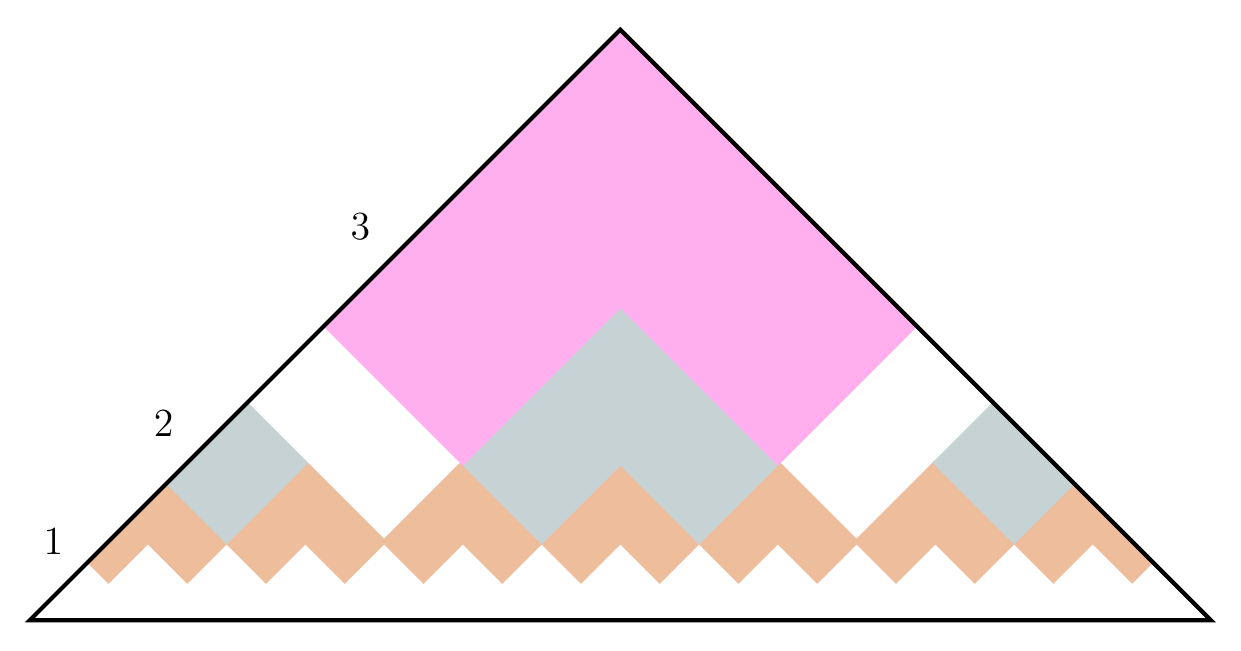
\begin{tikzpicture}[line width=1.5pt]
  % Треугольник таблицы
  \coordinate (BL)  at (0.5,0.5);
  \coordinate (BR)  at (15.5,0.5);
  \coordinate (TOP) at (8,8);

  \begin{scope}
    \clip (BL) -- (BR) -- (TOP) -- cycle;

    % Ряд 1: белые ромбы G(x,1), x = 1, 3, ..., 15 (15 штук)
    \foreach \x in {1,3,...,15} {
      \fill[white, draw] (\x,0.5) -- (\x-0.5,1) -- (\x,1.5) -- (\x+0.5,1) -- cycle;
    }

    % Ряд 2 (метка 1): оранжевые шевроны C(x,1), x = 2, 4, ..., 14 (7 штук)
    \foreach \x in {2,4,...,14} {
      \fill[LayerOrange, draw]
        (\x-0.5,1) -- (\x-1,1.5) -- (\x,2.5) -- (\x+1,1.5) -- (\x+0.5,1) -- (\x,1.5) -- cycle;
    }

    % Ряд 3 (метка 2): серые шевроны C(x,2), x = 2, 8, 14 (3 штуки)
    \foreach \x in {2,8,14} {
      \fill[LayerGray, draw]
        (\x-1,1.5) -- (\x-2,2.5) -- (\x,4.5) -- (\x+2,2.5) -- (\x+1,1.5) -- (\x,2.5) -- cycle;
    }

    % Ряд 4 (метка 3): розовый шеврон C(8,4)
    \fill[LayerPink, draw]
      (6,2.5) -- (4,4.5) -- (8,8.5) -- (12,4.5) -- (10,2.5) -- (8,4.5) -- cycle;
  \end{scope}

  % Контур треугольника (поверх обрезанных фигур)
  \draw (BL) -- (BR) -- (TOP) -- cycle;

  % Метки рядов слева от треугольника (на расстоянии ~1 единицы от левого края)
  \node[font=\Large] at (0.8,1.5) {1};
  \node[font=\Large] at (2.2,3)   {2};
  \node[font=\Large] at (4.7,5.5) {3};
\end{tikzpicture}
